% Author: David Paulino
% Date: 2023-03-03
% Description: LaTeX Template
% Vous êtes libre de modifier/ajouter de nouvelles commandes dans le fichier ou même de nouveau packages.

\documentclass[12pt]{article}

% Document en français
\usepackage[french]{babel}

% Color on table
\usepackage[table,xcdraw]{xcolor}

\usepackage[utf8]{inputenc}
\usepackage[T1]{fontenc}
\usepackage{graphicx}
\usepackage{amsmath}
\usepackage{amssymb}
\usepackage{amsthm}
\usepackage{amsfonts}
\usepackage{amscd}
\usepackage{amstext}

\usepackage{hyperref}
\usepackage{xcolor}
\usepackage{fancyhdr}
\usepackage{setspace}
\usepackage{float}
\usepackage{subfig}
\usepackage{caption}
\usepackage{listings}
\usepackage{tikz}
\usepackage{pgfplots}
\usepackage{pgfplotstable}
\usepackage{pgf}

% Add references in table of contents
\usepackage[nottoc]{tocbibind}

% Set author and place
% TODO: Changer les valeurs ci-dessous
% Elle seront utilisées pour la page de titre et les en-têtes/pieds de page
\newcommand{\authorname}{John Doe}
\newcommand{\place}{Genève}
\newcommand{\fulltitle}{Le titre complet du travail de bachelor}
\newcommand{\shorttitle}{Titre raccourci du travail}

% On retire l'indentation des paragraphes
\setlength{\parindent}{0pt}
% Augmentation de l'espacement entre les sauts de ligne
%\setlength{\parskip}{5pt} % Modifier la valeur selon vos besoins

% Title
\title{\fulltitle}
\author{\authorname}
\date{\today}

% Header
\pagestyle{fancy}
\fancyhf{}
\renewcommand{\headrulewidth}{0pt}
\lhead{\authorname}
\rhead{\shorttitle}

% Footers
\lfoot{Page \thepage}
\rfoot{\today}

% Document
\begin{document}

% Title page
\begin{titlepage}

    \begin{figure}[h]
        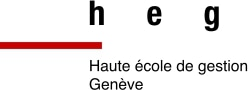
\includegraphics[width=0.3\textwidth]{img/logo_heg-ge.jpg}
    \end{figure}

    \vspace*{0.5cm}

    \begin{center}

        \begingroup \linespread{1,75} \selectfont
        {\Large \fulltitle}\\[0,75cm]
        \endgroup


        % Make a vertical space

        \vspace{1.5cm}

        \textsc{\large Travail de Bachelor HES réalisé en vue de \newline l’obtention du Bachelor par :}\\[0,50cm]

        \begingroup \linespread{1,5} \selectfont
        \textsc{\large \authorname}\\[0,50cm]
        \endgroup


        \vspace{1cm}


        \textsc{\large Conseillers au travail de Bachelor : }

        \begingroup \linespread{1,5} \selectfont
        \textsc{\large Pr Alexandros KALOUSIS}\\[0.1cm]
        \textsc{\large Dr Nils SCHÄTTI}\\[1cm]
        \endgroup


        \begingroup \linespread{1,75} \selectfont
        \textsc{\large \place, le \today}\\[0,1cm]

        {\large Haute école de Gestion de Genève (HEG-GE)}\\[0,1cm]

        {\large Filière Informatique de gestion}\\[0,1cm]
        \endgroup



        \begin{figure}[h]
            \vspace{0.05cm}
            \hspace*{12cm}
\includegraphics[width=0.25\textwidth]{img/logo_hes-so.jpg}
        \end{figure}

    \end{center}



    \vfill
\end{titlepage}




\newpage

\section{Déclaration}
% Insérer la déclaration ici
% Il est possible que 
Ce travail de Bachelor est réalisé dans le cadre de l'examen final de la Haute école de gestion de Genève, en vue de l'obtention du titre de Bachelor of Science HES-SO en Informatique de gestion.
\newline\newline
L'étudiant a envoyé ce document par email à l'adresse remise par son conseiller au travail de Bachelor pour analyse par le logiciel de détection de plagiat URKUND, selon la procédure détaillée à l'URL suivante : \url{https://www.urkund.com}
\newline\newline
L'étudiant accepte, le cas échéant, la clause de confidentialité.
L'utilisation des conclusions et recommendations formulées dans le travail de Bachelor, sans préjuger de leur valeur, n'engage ni la responsabilité de l'auteur, ni celle du conseiller au travail de Bachelor, du juré et de la HEG.
\newline\newline
"J'atteste avoir réalisé seul le présent travail, sans avoir utilisé des sources autres que celles citées dans la bibliographie."
% Faire un grand saut de ligne
\vspace{4cm}
% Aligner le texte à droite
\begin{flushright}
    Fait à \place, le \today
\end{flushright}

\begin{flushright}
    \authorname
\end{flushright}
\vspace{1cm}
\begin{flushright}
    --------------------------------
\end{flushright}


\newpage

\section{Remerciements}
% Insérer les remerciements ici
La partie où on remercie les gens qui nous ont aidé à réaliser ce travail de bachelor.

\newpage

\section{Résumé}
% Insérer le résumé ici
Voilà le résumé de ce travail de bachelor. Il est important de bien résumer le travail pour que le lecteur puisse comprendre le contenu de ce travail sans avoir à le lire en entier.


\newpage

% Liste des tableaux
\listoftables

\newpage

% Liste des figures
\listoffigures

\newpage

% Table of contents
\tableofcontents
\newpage

% Content
% Ce sont des exemples de sections, vous pouvez les modifier ou les supprimer

\section{Introduction}
\subsection{Exemple de création de liste}

Il est possible de créer des listes à puces ou numérotées.

\begin{itemize}
    \item Item 1
    \item Item 2
    \item Item 3
\end{itemize}

\begin{enumerate}
    \item Item 4
    \item Item 5
    \item Item 6
\end{enumerate}

\subsection{Exemple de création de tableau}
La création de tableau peut être faite en utilisant le site suivant : \url{https://www.tablesgenerator.com/}
\newline\newline
Il est ensuite possible de citer le tableau en utilisant la commande :
\textbf{\\ref\{labelDuTableau\}}.
\newline
Cela donne la référence vers le tableau \ref{tab:my-table}.
% Le htp permet de dire comment le tableau va être placé dans le document
% h = here, donc il va être placé à l'endroit où il est déclaré dans le code
% t = top, donc il va être placé en haut de la page si le h n'est pas possible
% p = page, donc il va être placé sur une page dédiée aux tableaux si le h et le t ne sont pas possibles
\begin{table}[htp]
    % On indique qu'on veut la centrer
    \centering
    \begin{tabular}{|l|l|l|}
        \hline
        \textbf{Colonne 1} & \textbf{Colonne 2} & \textbf{Colonne 3} \\ \hline
        Ligne 1            & Ligne 1            & Ligne 1            \\ \hline
        Ligne 2            & Ligne 2            & Ligne 2            \\ \hline
        Ligne 3            & Ligne 3            & Ligne 3            \\ \hline
    \end{tabular}
    % Légende du tableau
    \caption{Exemple de tableau simple}
    % Label du tableau
    \label{tab:my-table}
\end{table}

\begin{table}[htp]
    \centering
    \begin{tabular}{|ll|l|}
        \hline
        \multicolumn{2}{|c|}{\textbf{Couleur}}               & \textbf{Cellule 2}           \\ \hline
        \rowcolor[HTML]{FFCE93}
        \multicolumn{1}{|l|}{\cellcolor[HTML]{FFCE93}Orange} & 0                  & Texte   \\ \hline
        \rowcolor[HTML]{ECF4FF}
        \multicolumn{1}{|l|}{\cellcolor[HTML]{ECF4FF}Bleu}   & 1                  & Texte 2 \\ \hline
        \rowcolor[HTML]{CBCEFB}
        \multicolumn{1}{|l|}{\cellcolor[HTML]{CBCEFB}Violet} & 2                  & Texte 3 \\ \hline
        \rowcolor[HTML]{FFCCC9}
        \multicolumn{1}{|l|}{\cellcolor[HTML]{FFCCC9}Rouge}  & 3                  & Texte 4 \\ \hline
        \rowcolor[HTML]{FFFC9E}
        \multicolumn{1}{|l|}{\cellcolor[HTML]{FFFC9E}Jaune}  & 4                  & Texte 5 \\ \hline
    \end{tabular}
    \caption{Exemple de tableau avec couleurs}
    \label{tab:my-table-2}
\end{table}

\subsection{Exemple de création de figure}

Il est également possible de créer des figures. Il est possible de les citer en utilisant la commande :
\textbf{\\ref\{labelDeLaFigure\}}.
\newline
Cela donne la référence vers la figure \ref{fig:my-figure}.

\begin{figure}[htp]
    % On indique qu'on veut la centrer
    \centering
    % On indique la largeur de la figure, ici 50% de la largeur du texte
    % On peut indiquer également en cm, mm, in, etc.
    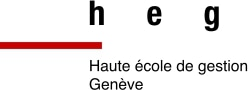
\includegraphics[width=0.5\textwidth]{img/logo_heg-ge.jpg}
    % Légende de la figure
    \caption{Exemple de figure}
    % Label de la figure
    \label{fig:my-figure}
\end{figure}

\subsection{Exemple de création de formule mathématique}

Il est possible de créer des formules mathématiques en utilisant la commande \textbf{\\begin\{equation\}}.
\newline
Cela donne la formule \ref{eq:my-equation}.
\begin{equation}
    \label{eq:my-equation}
    a^2 + b^2 = c^2
\end{equation}
Il est également possible d'écrire des formules mathématiques plus complexe, exemple avec la loi de Bayes \ref{eq:bayes} ou encore la loi gaussienne \ref{eq:gauss}.
\begin{equation}
    \label{eq:bayes}
    P(A|B) = \frac{P(B|A)P(A)}{P(B)}
\end{equation}

\begin{equation}
    \label{eq:gauss}
    f(x) = \frac{1}{\sigma\sqrt{2\pi}}e^{-\frac{1}{2}\left(\frac{x-\mu}{\sigma}\right)^2}
\end{equation}

N'hésitez pas à vous documenter pour écrire des formules mathématiques plus complexes.

\subsection{Exemple de citation de source}

Il est possible de citer des sources en utilisant la commande \textbf{\\cite\{labelDeLaSource\}}.
\newline
Cela donne la référence vers la source \cite{sumpterFittingXGModel}.
\newline
Il faut que la source soit dans le fichier \textbf{bibliography.bib}. Il est possible de faire cela à l'aide de Zotero pour créer la source et l'exporter dans le fichier \textbf{bibliography.bib}.
\newline
Une fois la source dans le fichier \textbf{bibliography.bib} et citée, elle sera ajoutée automatiquement dans la bibliographie à la fin du document.

\section{État de l'art}
\section{Méthodologie}
\section{Résultats}
\subsection{Sous-section des résultats}
\subsubsection{Sous-sous-section des résultats}

\section{Conclusion}


% Bibliography
% Il est possible d'afficher la bibliographie sous différentes formes en changeant le style
% Différents styles possibles : https://www.overleaf.com/learn/latex/Bibtex_bibliography_styles
\bibliographystyle{plainurl}
% Nom du fichier .bib
\bibliography{bibliography}

\end{document}